documentclass[border=0pt]{standalone}
\usepackage{tikz}
\usetikzlibrary{positioning}
\usetikzlibrary{shapes.geometric}
\usetikzlibrary{calc}
\begin{document}
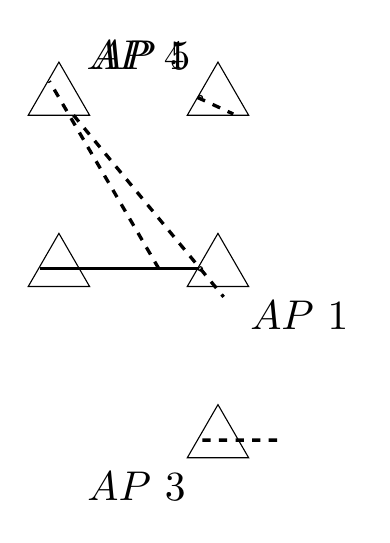
\begin{tikzpicture}[scale=1.5, every node/.style={transform shape},
    ap/.style={shape=regular polygon, regular polygon sides=3, draw=black,
            minimum size=6mm, inner sep=0mm, outer sep=0mm},
    user/.style={circle, draw=black, fill=gray!40, inner sep=0mm},
    line/.style={draw=black, very thick, shorten >=-5mm}]
    %AP
    \node[ap] (AP_1) {};
    \node[ap, right=of AP_1, label={[anchor=north west]south east:$\text{AP~1}$}] (AP_2) {};
    \node[ap, above=of AP_1, label={[anchor=south west]north east:$\text{AP~4}$}] (AP_3) {};
    \node[ap, above=of AP_2, label={[anchor=south east]north west:$\text{AP~5}$}] (AP_4) {};
    \node[ap, below=of AP_2, label={[anchor=north east]south west:$\text{AP~3}$}] (AP_5) {};

    %User
    \node[user, right=of AP_1] (U_1) {};
    \node[user, right=of AP_3] (U_2) {};

    %Line
    \draw[line] (U_1) -- (AP_1);
    \draw[line,dashed] ($(AP_2)+(-180:0.5)$) -- (AP_3);
    \draw[line,dashed] (AP_3) -- (U_1);
    \draw[line,dashed] (U_2) -- (AP_4);
    \draw[line,dashed] ($(AP_5)+(0:0.5)$) -- (AP_5);
\end{tikzpicture}
\end{document}